% palette (Paul Tol's vibrant set, colour-blind safe): one hue per device,
% and green / red / blue for the decoding outcome
\definecolor{irA}{HTML}{0077BB}
\definecolor{irB}{HTML}{EE7733}
\definecolor{irC}{HTML}{AA3377}
\definecolor{irD}{HTML}{009988}
\definecolor{irOk}{HTML}{228833}
\definecolor{irSic}{HTML}{0077BB}
\definecolor{irLost}{HTML}{CC3311}
\DeclareRobustCommand{\figIrsa}{%
\begin{figure}[t]
  \centering
  \begin{tikzpicture}[
      font=\footnotesize, x=0.8cm, y=0.85cm, >=stealth,
      slot/.style={draw=gray!50, minimum width=0.8cm, minimum height=0.4cm, inner sep=0pt},
      rep/.style={draw, rounded corners=1.5pt, minimum width=0.62cm, minimum height=0.27cm, inner sep=0pt, font=\bfseries, text=white},
      lbl/.style={anchor=east, inner sep=2pt},
      sic/.style={->, thick, dashed, irSic},
    ]
    % one row per device, one column per slot: a replica is a coloured box
    \foreach \k/\col in {1/irA, 2/irB, 3/irC, 4/irD} {
      \node[lbl, text=\col] at (0.45, {2.5-0.5*\k}) {\k};
      \foreach \s in {1,...,5} { \node[slot] at (\s, {2.5-0.5*\k}) {}; }
    }
    \foreach \s in {1,...,5} { \node[text=gray!40!black, anchor=south, inner sep=1pt] at (\s, 2.23) {\s}; }
    % axes: time slots to the right, devices downward
    \draw[->, gray!40!black] (0.5, 2.62) -- node[above, inner sep=1pt] {time slot} (5.5, 2.62);
    \draw[->, gray!40!black] (0.05, 2.3) -- (0.05, 0.2);
    \node[rotate=90, anchor=south, inner sep=1pt] at (-0.12, 1.25) {device};
    \node[rep, fill=irA] (a1) at (1, 2.0) {1};  \node[rep, fill=irA] (a2) at (3, 2.0) {1};
    \node[rep, fill=irB] (b1) at (2, 1.5) {2};  \node[rep, fill=irB] (b2) at (3, 1.5) {2};
    \node[rep, fill=irC] at (4, 1.0) {3};  \node[rep, fill=irC] at (5, 1.0) {3};
    \node[rep, fill=irD] at (4, 0.5) {4};  \node[rep, fill=irD] at (5, 0.5) {4};
    % decoded singletons cancel their other replica along the row
    \draw[sic] (a1.east) -- (a2.west);
    \draw[sic] (b1.east) -- (b2.west);
    % the outcome per slot
    \node[text=irOk] at (1, 0.05) {\faCheck};
    \node[text=irOk] at (2, 0.05) {\faCheck};
    \node[text=irSic] at (3, 0.05) {\faCheck\,\textbf{SIC}};
    \node[text=irLost] at (4, 0.05) {\faTimes};
    \node[text=irLost] at (5, 0.05) {\faTimes};
    % legend, in the space right of the frame
    \node[anchor=west, align=left, inner sep=0pt] at (5.65, 1.2) {%
      \textcolor{irOk}{\faCheck} singleton\\[3pt]
      \textcolor{irSic}{\faCheck\,\textbf{SIC}}\\[3pt]
      \textcolor{irLost}{\faTimes} collision};
  \end{tikzpicture}
  \caption{An IRSA frame of $M = 5$ slots with four packets of $L = 2$ replicas.}
  \label{fig:irsa}
\end{figure}%
}
